%% This is an example first chapter.  You should put chapter/appendix that you
%% write into a separate file, and add a line \include{yourfilename} to
%% main.tex, where `yourfilename.tex' is the name of the chapter/appendix file.
%% You can process specific files by typing their names in at the 
%% \files=
%% prompt when you run the file main.tex through LaTeX.

\singlespacing{

\chapter{Design Hierarchy}

Parts\\
Functions\\
Modules\\
Systems\\


\section{Parts}

At the lowest level, bulk materials in the form of \textit{parts} are assembled together to form multimaterial assemblies.  
Parts components are on the order of ~1um\textsuperscript{3}.

\section{Functions}

Assemblies of \textit{parts} form components called \textit{functions}.
Functional Components are on the order of ~1mm\textsuperscript{3}.

degrees of freedom (function) + interface

\section{Modules}

\section{Systems}

\section{Examples}

\subsection{Biology}

At the most fundamental level, biological structures are composed of atoms of various elemental types.  Each element's unique position on the periodic table dictates its mass, the number of covalent bonds it can form, the amount of unpaired electrons it contains in its outermost electron shell, the polarization of the bonds and molecules it forms with other elements, and the stability of its bonds in various environments.  These physical parameters have implications in higher-level structures formed from the elemental parts, called \textit{functional groups}.\\



In organic chemistry, functional groups are organized into a few archetypal categories \\

\begin{figure}
  \includegraphics[width=\textwidth]{AminosInterface.png}
  \caption{Decomposition of amino acids into carboxylic acid and amine interface (blue and pink) and function (orange).}
  \label{fig:AminosInterface}
\end{figure}

We can think of each of the amino acids as being composed of a standardized interface and a function.  The interface of an amino acid is formed by the carboxylic acid (COOH) and amine groups (NH\textsubscript{2}).  


\begin{figure}
  \includegraphics[width=\textwidth]{PeptideBond.png}
  \caption{Formation of peptide bond at c-terminus of polypeptide chain. One molecule of water is produced as a byproduct of the peptide bonding reaction.  R, R', and R'' represent arbitrary amino acid sidechains.}
  \label{fig:PeptideBond}
\end{figure}
PeptideBond


 that form the connections between amino acids in a polypeptide chain through peptide bonds.  Peptide bonding forms a covalent bond between two amino acids through a process called \textit{condensation}, where a single molecule of water is created as a byproduct.\\

In a process called \href{https://en.wikipedia.org/wiki/Translation_%28biology%29}{\textit{translation}}, amino acids are linked together to form protein chains in a cell.  During translation, the c-terminus (the carboxylic acid group) of the growing protein chain is connected to the n-terminus (the amine group) of the next animo acid.

\begin{sidewaysfigure}
  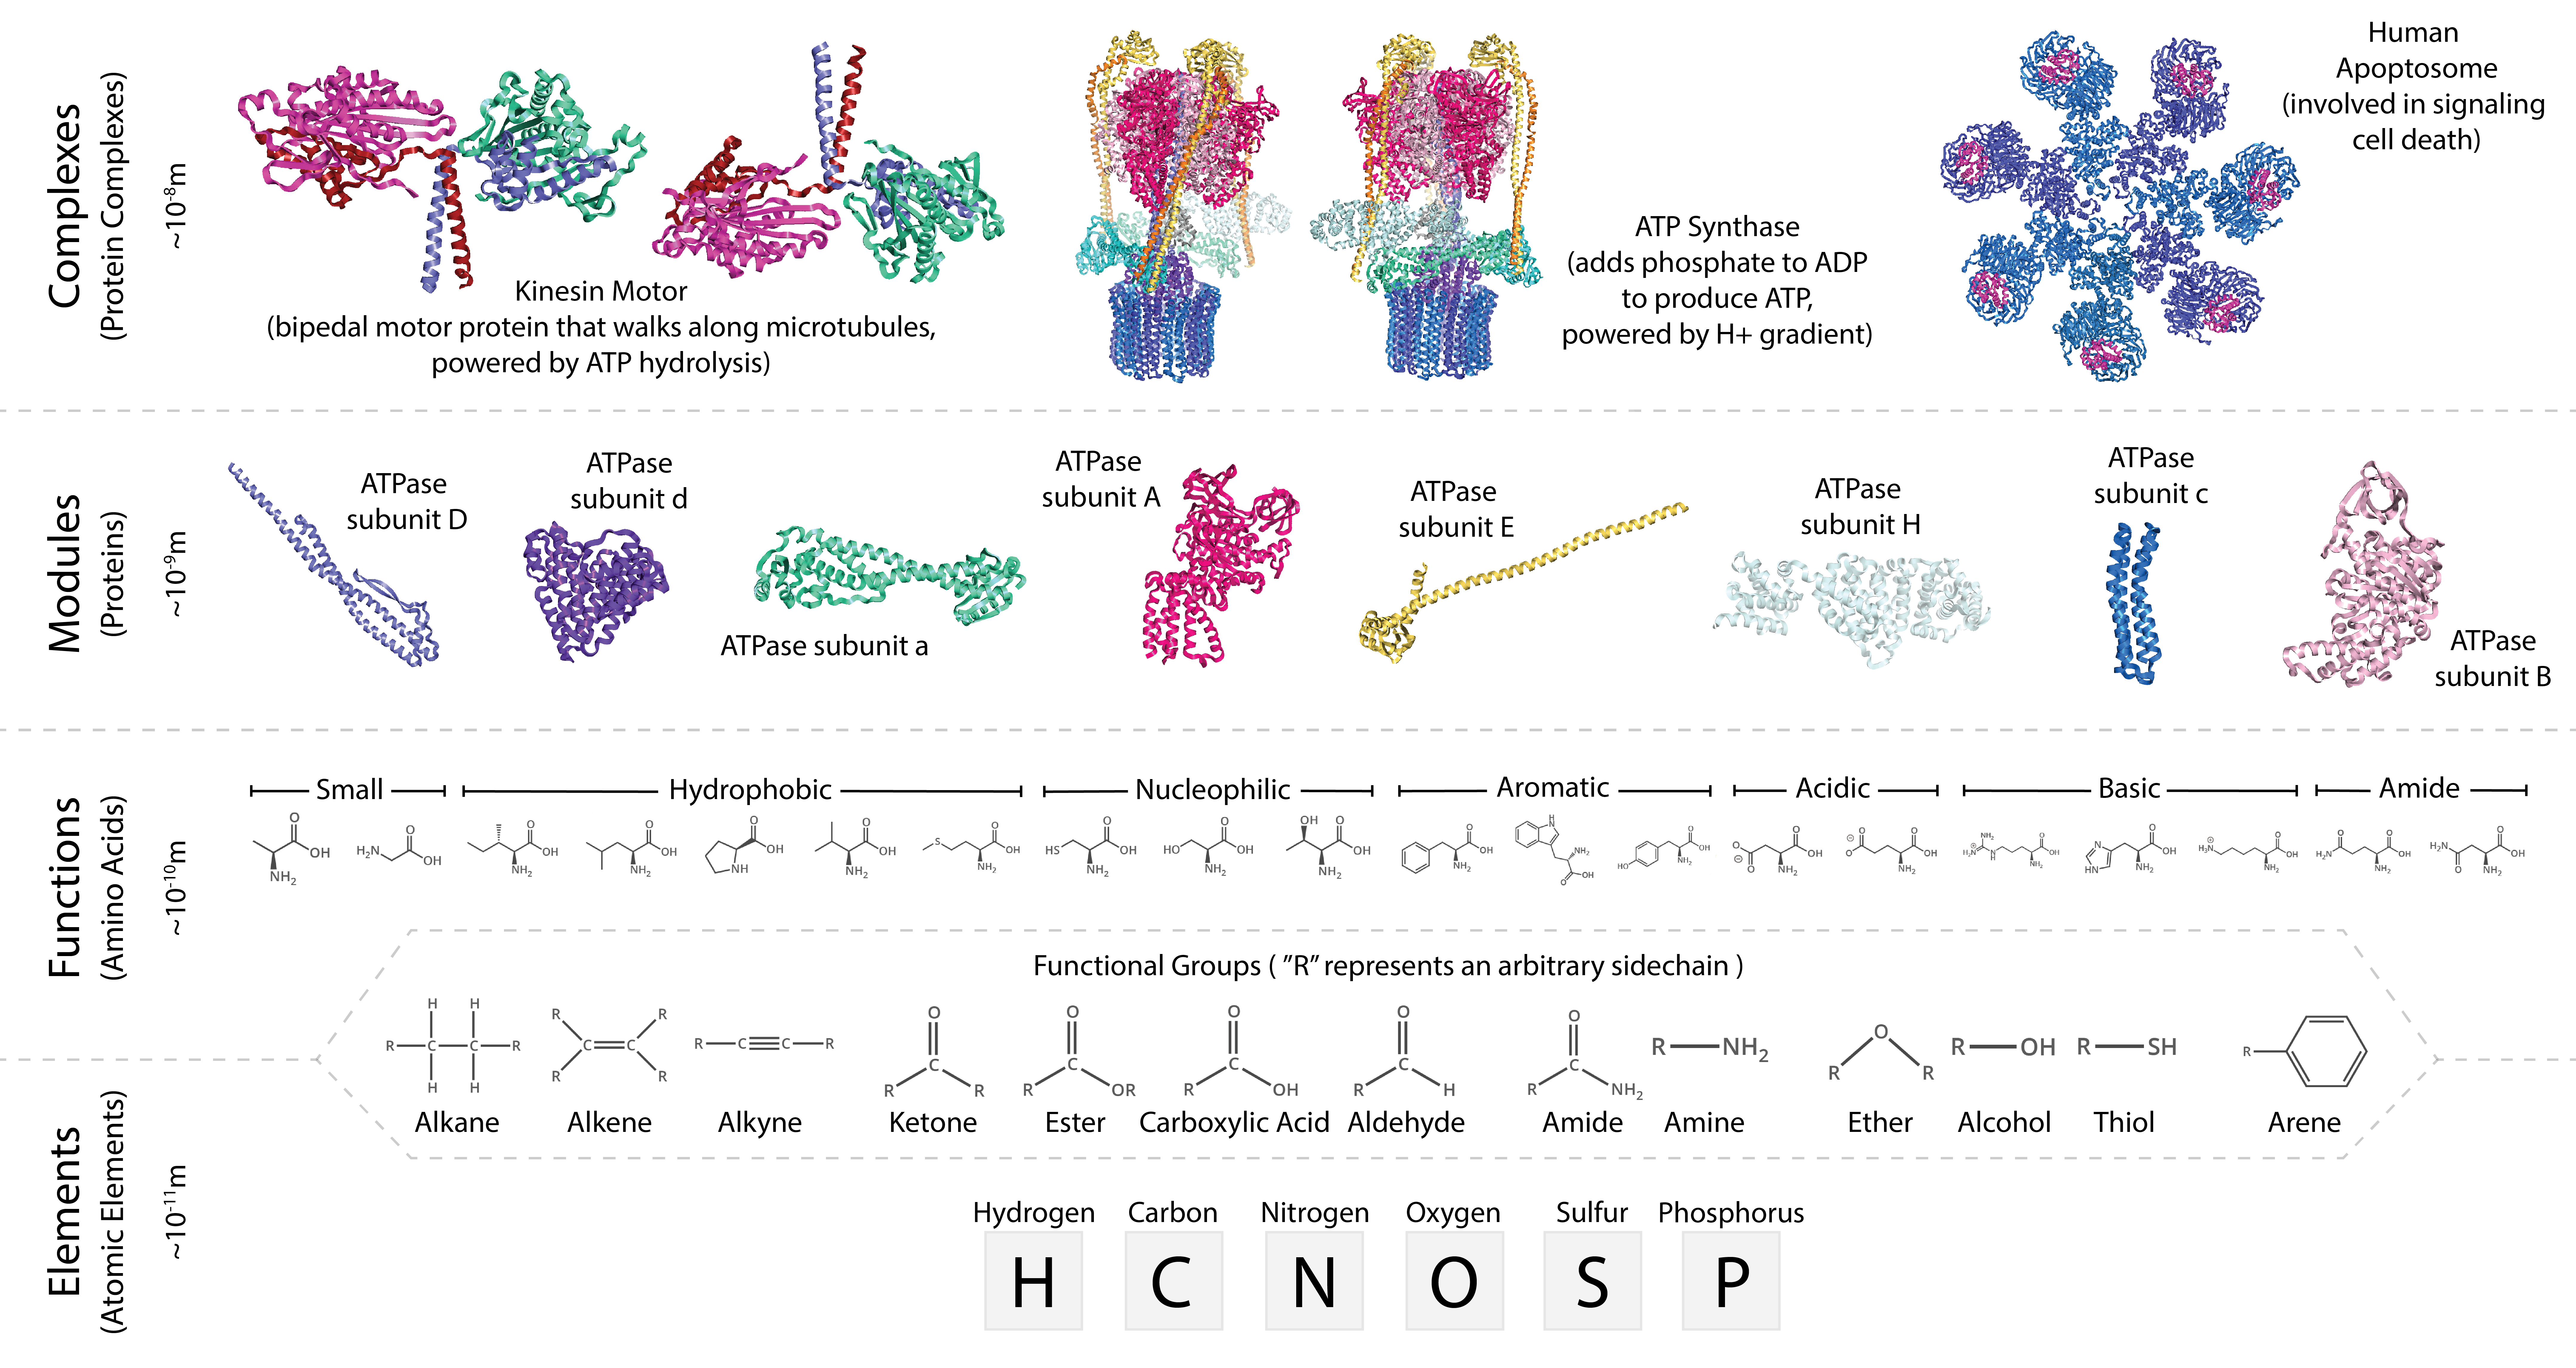
\includegraphics[width=\textwidth,height=\textheight,keepaspectratio]{ProteinHierarchy.png}
  \caption{Hierarchical breakdown of protein complexes into modules, functions, and parts.  Bulk elements}
  \label{fig:ProteinHierarchy}
\end{sidewaysfigure}

\subsection{Conway's Game of Life}

\begin{figure}
  \includegraphics[width=\textwidth]{OTCADiagram.png}
  \caption{System level diagram of OTCA Metapixel with the most important modules highlighted.}
  \label{fig:OTCADiagram}
\end{figure}

\begin{sidewaysfigure}
  \includegraphics[width=\textwidth,height=\textheight,keepaspectratio]{OTCAMetaHierarchy.png}
  \caption{Hierarchical breakdown of OTCA Metapixel.}
  \label{fig:OTCAMetaHierarchy}
\end{sidewaysfigure}

\subsection{Von Neuman Universal Constructor}

\section{Exceptions}

scaling mismatch between the functional density of electronic and mechanical systems, offset in hierarchical setup.

\section{Hierarchy in Simulation}

increasing simulation abstraction as hierarchical level increases\\

In the next chapters, I'll describe the methods used to simulate parts and functions, and describe how abstractions of the parts-level simulation are adapted to the functions-level.



}
